% Exercises for Lesson 11: Advanced TikZ & PGFPlots
% Topic: LaTeX
% Solutions to practice problems from the lesson.
% Compile: pdflatex exercises/LaTeX/11_tikz_advanced.tex

\documentclass[12pt, a4paper]{article}
\usepackage[utf8]{inputenc}
\usepackage[T1]{fontenc}
\usepackage{amsmath, amssymb}
\usepackage{tikz}
\usepackage{pgfplots}
\pgfplotsset{compat=1.18}
\usetikzlibrary{
  arrows.meta, positioning, shapes.geometric,
  decorations.pathmorphing, decorations.pathreplacing,
  automata, calc
}

\title{Exercises for Lesson 11: Advanced TikZ \& PGFPlots}
\author{Study Project}
\date{}

\begin{document}
\maketitle

% === Exercise 1: Function Comparison ===
% Problem: Plot x^2, 2^x, log(x) on [0.1,5].

\section*{Exercise 1: Function Comparison}

\begin{center}
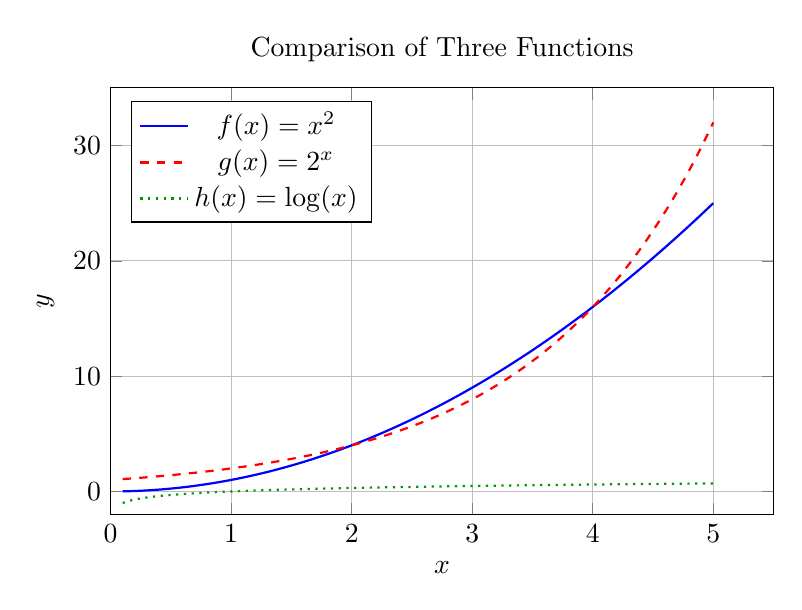
\begin{tikzpicture}
\begin{axis}[
  width=10cm, height=7cm,
  domain=0.1:5, samples=100,
  xlabel={$x$}, ylabel={$y$},
  title={Comparison of Three Functions},
  legend pos=north west,
  grid=major,
  xmin=0, xmax=5.5,
  ymin=-2, ymax=35
]
  \addplot[blue, thick]   {x^2};
  \addplot[red, thick, dashed]    {2^x};
  \addplot[green!60!black, thick, dotted] {ln(x)/ln(10)};
  \legend{$f(x) = x^2$, $g(x) = 2^x$, $h(x) = \log(x)$}
\end{axis}
\end{tikzpicture}
\end{center}

% === Exercise 2: Bar Chart ===
% Problem: Sales data, 6 categories, values on bars, custom colors.

\section*{Exercise 2: Bar Chart with Sales Data}

\begin{center}
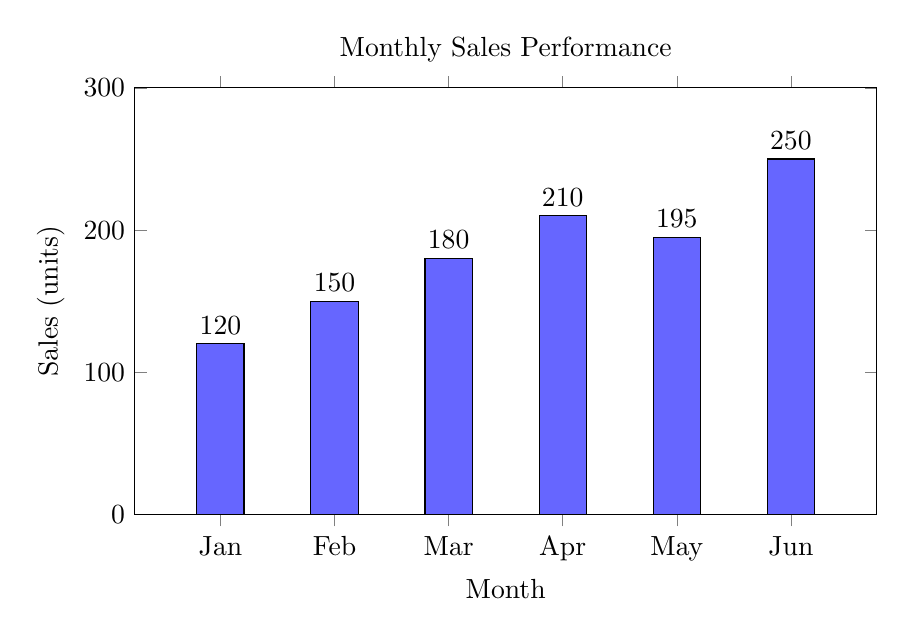
\begin{tikzpicture}
\begin{axis}[
  ybar,
  width=11cm, height=7cm,
  bar width=0.6cm,
  xlabel={Month},
  ylabel={Sales (units)},
  title={Monthly Sales Performance},
  symbolic x coords={Jan, Feb, Mar, Apr, May, Jun},
  xtick=data,
  nodes near coords,
  nodes near coords align={vertical},
  ymin=0, ymax=300,
  enlarge x limits=0.15,
]
  \addplot[fill=blue!60] coordinates {
    (Jan,120) (Feb,150) (Mar,180) (Apr,210) (May,195) (Jun,250)
  };
\end{axis}
\end{tikzpicture}
\end{center}

% === Exercise 3: 3D Surface Plot ===
% Problem: z = sin(x)cos(y), colormap, colorbar.

\section*{Exercise 3: 3D Surface Plot}

\begin{center}
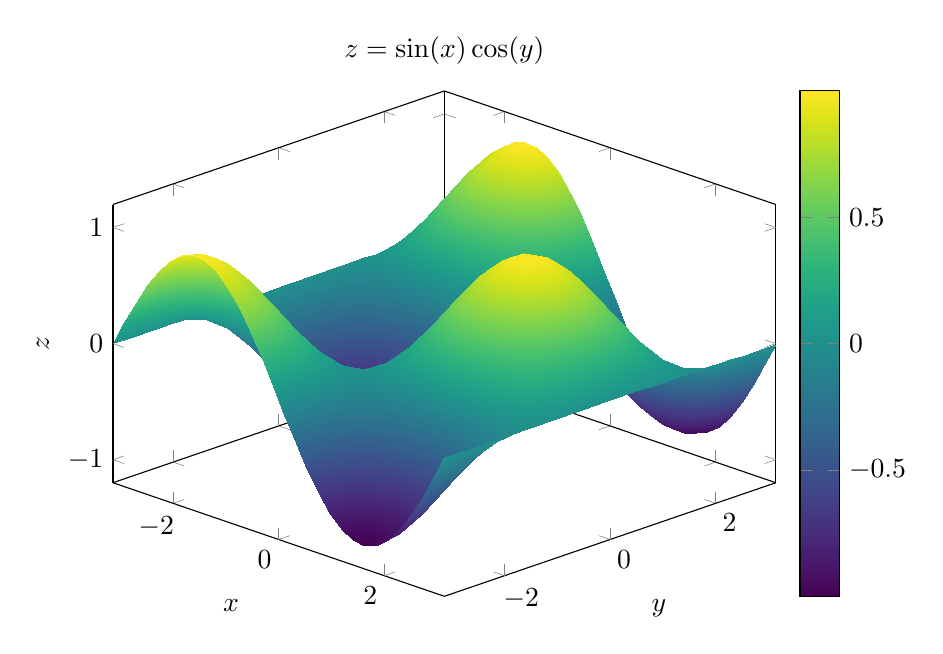
\begin{tikzpicture}
\begin{axis}[
  width=10cm, height=8cm,
  view={45}{30},
  xlabel={$x$}, ylabel={$y$}, zlabel={$z$},
  title={$z = \sin(x)\cos(y)$},
  colormap/viridis,
  colorbar,
  domain=-3.14:3.14,
  y domain=-3.14:3.14,
  samples=30,
]
  \addplot3[surf, shader=interp] {sin(deg(x))*cos(deg(y))};
\end{axis}
\end{tikzpicture}
\end{center}

% === Exercise 4: Foreach Grid / Checkerboard ===
% Problem: 8x8 checkerboard with alternating colors.

\section*{Exercise 4: Checkerboard Pattern}

\begin{center}
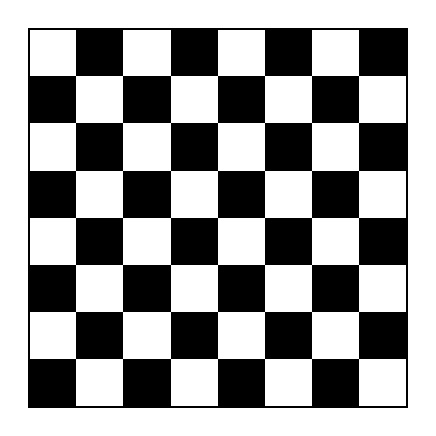
\begin{tikzpicture}[scale=0.6]
  \foreach \row in {0,...,7} {
    \foreach \col in {0,...,7} {
      \pgfmathparse{mod(\row+\col,2) ? "white" : "black"}
      \edef\squarecolor{\pgfmathresult}
      \fill[\squarecolor] (\col, \row) rectangle (\col+1, \row+1);
    }
  }
  \draw[thick] (0,0) rectangle (8,8);
\end{tikzpicture}
\end{center}

% === Exercise 5: Binary Tree ===
% Problem: 3 levels, 7 nodes, circular, numbered 1-7, colored by level.

\section*{Exercise 5: Binary Tree}

\begin{center}
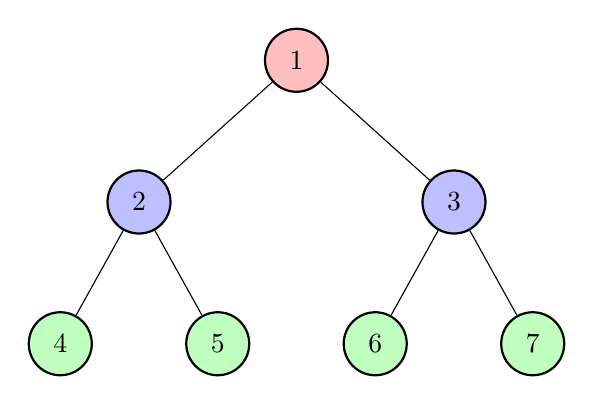
\begin{tikzpicture}[
  level 1/.style={sibling distance=4cm, level distance=1.8cm},
  level 2/.style={sibling distance=2cm, level distance=1.8cm},
  every node/.style={circle, draw, thick, minimum size=0.8cm},
]
  \node[fill=red!25] {1}
    child { node[fill=blue!25] {2}
      child { node[fill=green!25] {4} }
      child { node[fill=green!25] {5} }
    }
    child { node[fill=blue!25] {3}
      child { node[fill=green!25] {6} }
      child { node[fill=green!25] {7} }
    };
\end{tikzpicture}
\end{center}

% === Exercise 6: Decorated Diagram ===
% Problem: Beam rectangle, brace decorations, spring, force arrows.

\section*{Exercise 6: Decorated Beam Diagram}

\begin{center}
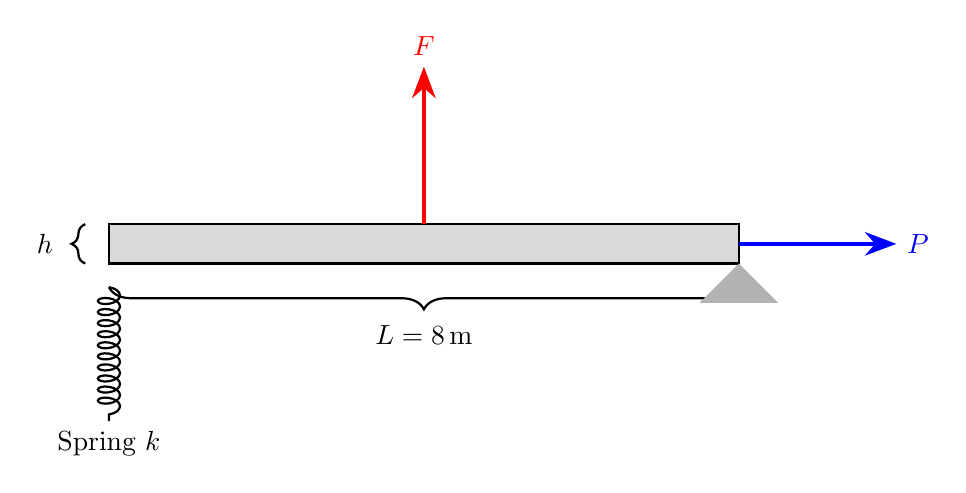
\begin{tikzpicture}
  % Beam
  \fill[gray!30] (0,0) rectangle (8,0.5);
  \draw[thick] (0,0) rectangle (8,0.5);

  % Brace for length
  \draw[decorate, decoration={brace, amplitude=8pt, mirror}, thick]
    (0,-0.3) -- (8,-0.3) node[midway, below=10pt] {$L = 8\,\text{m}$};

  % Brace for height
  \draw[decorate, decoration={brace, amplitude=5pt}, thick]
    (-0.3,0) -- (-0.3,0.5) node[midway, left=8pt] {$h$};

  % Spring on left support
  \draw[decorate, decoration={coil, segment length=4pt, amplitude=4pt},
    thick] (0,-0.3) -- (0,-2) node[below] {Spring $k$};

  % Force arrows
  \draw[-{Stealth[length=4mm]}, red, very thick]
    (4,0.5) -- (4,2.5) node[above] {$F$};
  \draw[-{Stealth[length=4mm]}, blue, very thick]
    (8,0.25) -- (10,0.25) node[right] {$P$};

  % Support triangle on right
  \fill[gray!60] (8,-0.5) -- (7.5,-0.5) -- (8,0) -- (8.5,-0.5) -- cycle;
\end{tikzpicture}
\end{center}

% === Exercise 7: Neural Network ===
% Problem: 3 input, 2 hidden layers (4 each), 2 output, all connections.

\section*{Exercise 7: Neural Network}

\begin{center}
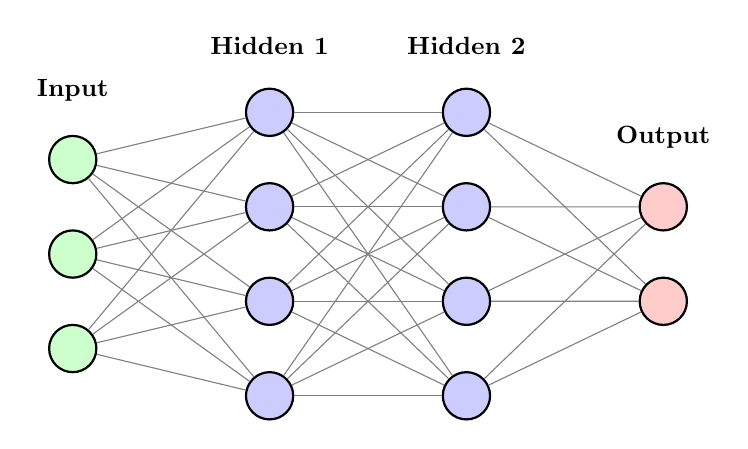
\begin{tikzpicture}[
  node distance=1.2cm,
  neuron/.style={circle, draw, thick, minimum size=0.6cm},
  input/.style={neuron, fill=green!20},
  hidden/.style={neuron, fill=blue!20},
  output/.style={neuron, fill=red!20},
]
  % Input layer
  \foreach \i in {1,2,3} {
    \node[input] (I\i) at (0, -\i*1.2) {};
  }
  \node[above=0.3cm of I1, font=\small\bfseries] {Input};

  % Hidden layer 1
  \foreach \j in {1,2,3,4} {
    \node[hidden] (H1\j) at (2.5, -\j*1.2 + 0.6) {};
  }
  \node[above=0.3cm of H11, font=\small\bfseries] {Hidden 1};

  % Hidden layer 2
  \foreach \j in {1,2,3,4} {
    \node[hidden] (H2\j) at (5, -\j*1.2 + 0.6) {};
  }
  \node[above=0.3cm of H21, font=\small\bfseries] {Hidden 2};

  % Output layer
  \foreach \k in {1,2} {
    \node[output] (O\k) at (7.5, -\k*1.2 - 0.6) {};
  }
  \node[above=0.3cm of O1, font=\small\bfseries] {Output};

  % Connections: input -> hidden 1
  \foreach \i in {1,2,3} {
    \foreach \j in {1,2,3,4} {
      \draw[thin, gray] (I\i) -- (H1\j);
    }
  }

  % Connections: hidden 1 -> hidden 2
  \foreach \i in {1,2,3,4} {
    \foreach \j in {1,2,3,4} {
      \draw[thin, gray] (H1\i) -- (H2\j);
    }
  }

  % Connections: hidden 2 -> output
  \foreach \i in {1,2,3,4} {
    \foreach \k in {1,2} {
      \draw[thin, gray] (H2\i) -- (O\k);
    }
  }
\end{tikzpicture}
\end{center}

% === Exercise 8: State Machine ===
% Problem: 4+ states, initial, accepting, transitions with self-loops.

\section*{Exercise 8: Finite State Automaton}

\begin{center}
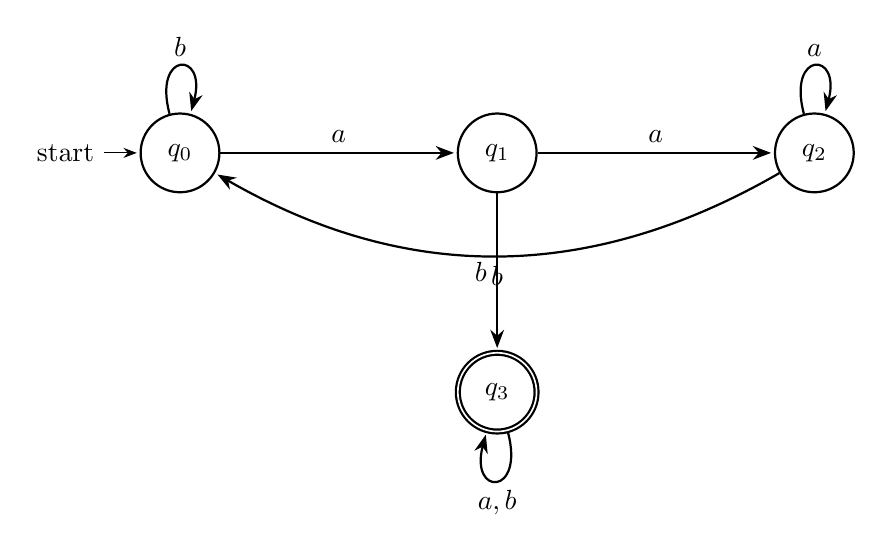
\begin{tikzpicture}[
  ->, >=Stealth, shorten >=1pt,
  node distance=3cm,
  every state/.style={thick, minimum size=1cm},
  auto
]
  \node[state, initial]           (q0) {$q_0$};
  \node[state, right=of q0]      (q1) {$q_1$};
  \node[state, right=of q1]      (q2) {$q_2$};
  \node[state, accepting, below=2cm of q1] (q3) {$q_3$};

  \path[thick]
    (q0) edge node {$a$}     (q1)
    (q0) edge [loop above] node {$b$} (q0)
    (q1) edge node {$a$}     (q2)
    (q1) edge node [swap] {$b$} (q3)
    (q2) edge [loop above] node {$a$} (q2)
    (q2) edge [bend left] node {$b$} (q0)
    (q3) edge [loop below] node {$a,b$} (q3);
\end{tikzpicture}
\end{center}

% === Exercise 9: Multi-Panel Plot ===
% Problem: 2 side-by-side plots -- scatter with error bars, line with fill.

\section*{Exercise 9: Multi-Panel Plot}

\begin{center}
\begin{tikzpicture}
\begin{axis}[
  name=left plot,
  width=6.5cm, height=6cm,
  xlabel={$x$}, ylabel={$y$},
  title={Scatter with Error Bars},
  grid=major,
]
  \addplot+[only marks, error bars/.cd, y dir=both, y explicit]
    coordinates {
      (1, 2.1) +- (0, 0.3)
      (2, 3.8) +- (0, 0.5)
      (3, 5.2) +- (0, 0.4)
      (4, 7.1) +- (0, 0.6)
      (5, 8.9) +- (0, 0.4)
    };
\end{axis}

\begin{axis}[
  at={(left plot.east)}, anchor=west, xshift=1.5cm,
  width=6.5cm, height=6cm,
  xlabel={$x$}, ylabel={$y$},
  title={Line with Confidence Interval},
  grid=major,
]
  % Upper bound
  \addplot[name path=upper, draw=none]
    coordinates {(0,1.5) (1,2.8) (2,4.5) (3,5.8) (4,7.2) (5,9.0)};
  % Lower bound
  \addplot[name path=lower, draw=none]
    coordinates {(0,0.5) (1,1.2) (2,2.5) (3,3.8) (4,5.2) (5,7.0)};
  % Fill between
  \addplot[blue!20] fill between[of=upper and lower];
  % Mean line
  \addplot[blue, thick]
    coordinates {(0,1.0) (1,2.0) (2,3.5) (3,4.8) (4,6.2) (5,8.0)};
\end{axis}
\end{tikzpicture}
\end{center}

% === Exercise 10: Publication Figure ===
% Problem: Publication-quality line plot with error bars, legend,
% grid, font sizes, 12cm width.

\section*{Exercise 10: Publication-Quality Figure}

\begin{center}
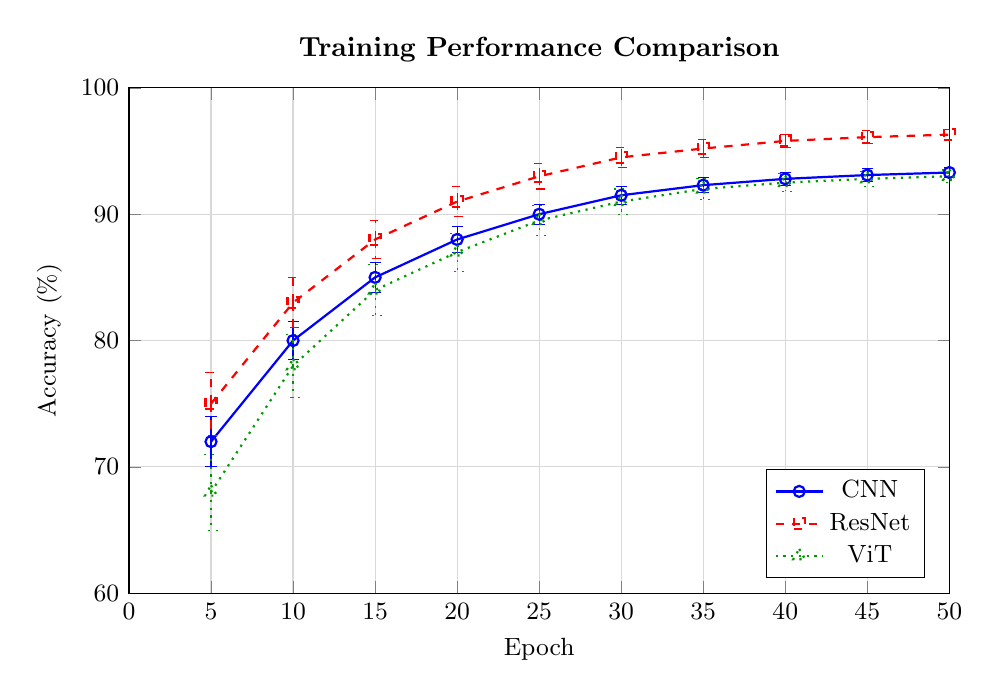
\begin{tikzpicture}
\begin{axis}[
  width=12cm, height=8cm,
  xlabel={Epoch},
  ylabel={Accuracy (\%)},
  title={Training Performance Comparison},
  legend pos=south east,
  legend style={font=\small},
  grid=both,
  minor grid style={gray!15},
  major grid style={gray!30},
  tick label style={font=\small},
  label style={font=\small},
  title style={font=\normalsize\bfseries},
  xmin=0, xmax=50, ymin=60, ymax=100,
]
  % Model A
  \addplot+[blue, thick, mark=o, mark size=2pt,
    error bars/.cd, y dir=both, y explicit]
    coordinates {
      (5,72) +- (0,2)   (10,80) +- (0,1.5)
      (15,85) +- (0,1.2) (20,88) +- (0,1)
      (25,90) +- (0,0.8) (30,91.5) +- (0,0.7)
      (35,92.3) +- (0,0.6) (40,92.8) +- (0,0.5)
      (45,93.1) +- (0,0.5) (50,93.3) +- (0,0.4)
    };

  % Model B
  \addplot+[red, thick, mark=square, mark size=2pt, dashed,
    error bars/.cd, y dir=both, y explicit]
    coordinates {
      (5,75) +- (0,2.5)  (10,83) +- (0,2)
      (15,88) +- (0,1.5) (20,91) +- (0,1.2)
      (25,93) +- (0,1)   (30,94.5) +- (0,0.8)
      (35,95.2) +- (0,0.7) (40,95.8) +- (0,0.5)
      (45,96.1) +- (0,0.5) (50,96.3) +- (0,0.4)
    };

  % Model C
  \addplot+[green!60!black, thick, mark=triangle, mark size=2.5pt, dotted,
    error bars/.cd, y dir=both, y explicit]
    coordinates {
      (5,68) +- (0,3)   (10,78) +- (0,2.5)
      (15,84) +- (0,2)  (20,87) +- (0,1.5)
      (25,89.5) +- (0,1.2) (30,91) +- (0,1)
      (35,92) +- (0,0.8)   (40,92.5) +- (0,0.7)
      (45,92.8) +- (0,0.6) (50,93.0) +- (0,0.5)
    };

  \legend{CNN, ResNet, ViT}
\end{axis}
\end{tikzpicture}
\end{center}

\end{document}
